\chapter{Simulation methods and results}
\label{chap:simulation}

In this chapter we present simulations performed with the objective of both gaining insight into the behavior of discrete phase
oscillators governed by the dynamics of (\ref{eq:rate}) and (\ref{eq:motion}), and to test predictions given by the  MF description
derived in chapter \ref{chap:mf}.  Computations were carried out at the Statistics and Computation Service (SCS) cluster at the
University of Michigan as well as local office and personal computers at UMICH and the University of Minas Gerais, and its source code
is publicly available as a \href{https://github.com/KiloLiuton/event-driven-cpp-minimalist}{git repository}\footnotemark{} for viewing
or recreating the data shown in this chapter. We start by defining the method chosen and exposing its implementation details, and then
move on to inspect the results produced.

\footnotetext{https://github.com/KiloLiuton/event-driven-cpp-minimalist}

\section{Event-driven simulation}

The system of discrete oscillators is a dynamical system where each oscillator has three possible phase values which can advance
forward to the next state. The rates with which they transition depend on the relative states between each unit and its coupled
neighbors through equation~(\ref{eq:rate}), leading to the set of equations of motion~(\ref{eq:motion}). We seek to define an update
rule for such a system that corresponds to solving these sets of equations.

The model structure over which the dynamics will act starts with some graph that defines the coupling between oscillators where nodes
represent oscillators and edges represent their coupling strength. Each node is labeled with a coordinate $x$ and the value associated
with it is it's phase state, encoded with the numbers 0, 1 and 2. The value associated with the edges is the coupling strength $a$,
which is the same for every edge. The next step is giving every oscillator an initial phase value, making the system well defined for
the dynamical rules to act on it.

The implementation of choice for applying the dynamical rules is the event driven method, where every update in the simulation is
guaranteed to contain exactly one event, which in this case constitutes an oscillator advancing to its next phase state. This method is
adequate here because the overall transition rate of the system, given by the sum of all individual transition rates, can vary by
several orders of magnitude depending on the systems macro state. Therefore, when the system is in a very ``quiet'' state with few
transitions happening, the simulation doesn't actually slow down, as would be the case in a simulation with fixed time step. Instead,
we dynamically widen the time step and ``fast forward'' to the next transition. On the other hand, if the simulation is in a very
active state, the event driven method prevents the scenario where too many oscillators would transition concurrently in the same time
step by reducing it, making the dynamics more representative of the actual equations they model. The price of these upsides is that the
dynamic calculation of the time step becomes the greatest computational cost in processing time, and it also makes computational
concurrency harder or even impossible to implement.

\subsection*{Calculating the simulation time step}

Each oscillator has a transition rate $\gamma^x$, such that the expected time elapsed until its next transition is $(\gamma^x)^{-1}$.
Since there are $N$ such units in the system, the average waiting time $\tau$ for any such event to occur is given by $\tau =
\Gamma^{-1}$ where $\Gamma \equiv \sum_x \gamma^x$ and therefore.

\begin{equation}
	\tau(t) = \frac{1}{\sum\limits_{x=1}^N \gamma^x(t)}
\end{equation}

\noindent where we have explicitly written the time dependence of the transition rates to show that the time step in the simulation is
also time dependent, increasing when the overall transition is small and slowing down when activity rises.

\subsection*{Algorithm}

Now that we know how to obtain the time step $\tau$, the average time elapsed until \textit{some} oscillator transitions, we need to
determine \textit{which} one actually underwent phase change. This is accomplished by sampling the transition rate distribution $r$
given by

\begin{equation}
	r(x,t_i)=\frac{\gamma^x(t_i)}{\Gamma(t_i)}
\end{equation}

\noindent at the current simulation time $t_i$. After sampling, the selected position $x$ is the label of the oscillator in the graph
that will be updated to its next phase value. Once the state is updated, we also need to update the transition rate $\gamma^x$ as well
as $\gamma^{x'}$ where $x'$ is a neighbor of $x$, allowing us to calculate the next time step $\tau(t_{i+1})$ and the new distribution
$r(x,t_{i+1})$. With these definitions the core loop procedure can be written as:

\begin{enumerate}
	\item Sample the distribution $r(x,t_i)$ to obtain the transitioning oscillators label $x$
	\item Update the phase value $\phi^x(t_i) \to \phi^x(t_{i+1})$ and rate $\gamma^x(t_i) \to \gamma^x(t_{i+1})$
	\item For all neighbors of $x$, update their respective rate values $\gamma^{x'}(t_i) \to \gamma^{x'}(t_{i+1})$
	\item Increment the simulation time by $\tau(t_i)$ such that $t_{i+1} = t_i + \tau(t_i)$
	\item If $t_{i}$ is larger than the desired simulation time, stop, otherwise, repeat from 1.
\end{enumerate}

Note that there is exactly one transition per iteration of the core loop, regardless of the value of $\tau(t_i)$.

Because calculating $\gamma(t_{i+1})$ requires comparing the new state $\phi(t_{i+1})$ to all of its neighbors, and because for each of
them only the state of $x$ has changed, there is some minor computational gain in combining steps 2 and 3, requiring a single loop
through the neighbors of $x$.

\section{Wave stability}

Travelling waves are not the only stable solution on ring lattices. In the mean field description, the only way a system may reach this
state is through a favorable initial condition. In real finite systems or in simulations this state may be reached spontaneously
through fluctuations, even if the system is already at some other stable configuration. Nonetheless, in order to facilitate the
stability study of wave solutions, we give the system an initial configuration that is already a wave. The MF description suggests that
some combinations of interaction range $\alpha$ and rewiring probability $p$ favors wave solutions through the equation for the
critical coupling $a_c$ for waves with wave number $m$:

\begin{align}
	a_c = \frac{3}{2}\frac{1}{(1-p)}\frac{(2\pi m\alpha)}{\sin(2\pi m\alpha)}
	\label{eq:critical_plane}
\end{align}

In chapter \ref{chap:article} we see that the critical coupling value for transitions to global synchrony does not change with $\alpha$
(figure~\ref{fig:chicurves} for example). In the case of wave configurations the critical value changes with connectivity as well as
wave number $m$. In addition, the introduction of disorder through the rewiring probability $p$ also affects the stability of wave
solutions according to equation~(\ref{eq:critical_plane}) (at least for small $p$), but this effect is minor when compared to the
effect it has on the onset of global synchrony or the infinite period transition, as seen from figure~\ref{fig:chicurvespvalue}, where
a very small amount of disorder causes wave solutions to quickly destabilize, giving way to global oscillations and infinite period
steady states.

\begin{figure}
  \centering
  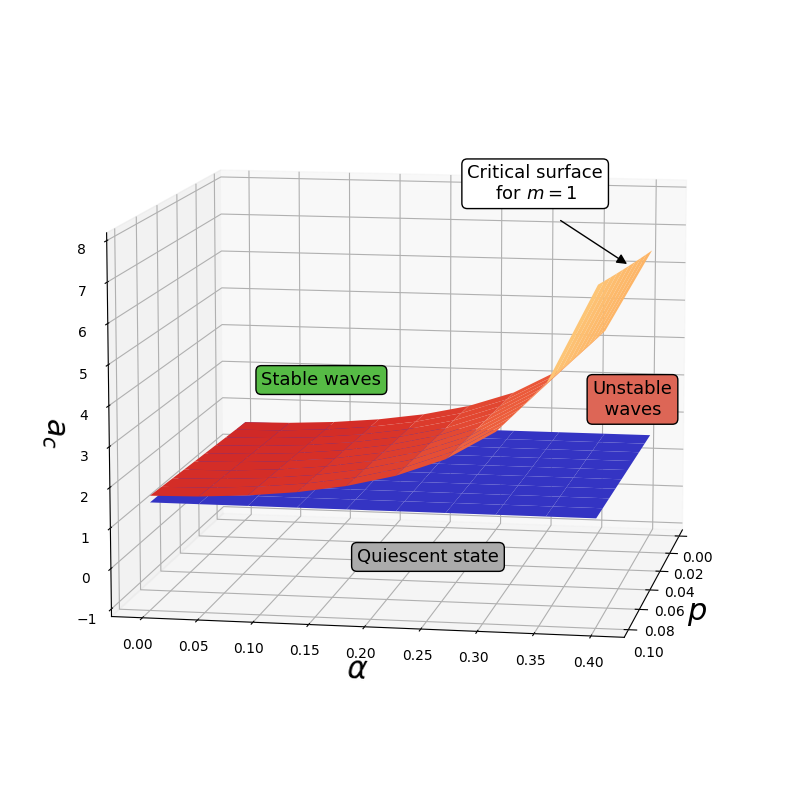
\includegraphics[width=0.45\textwidth]{fig/chap4/critical_plane.png}
  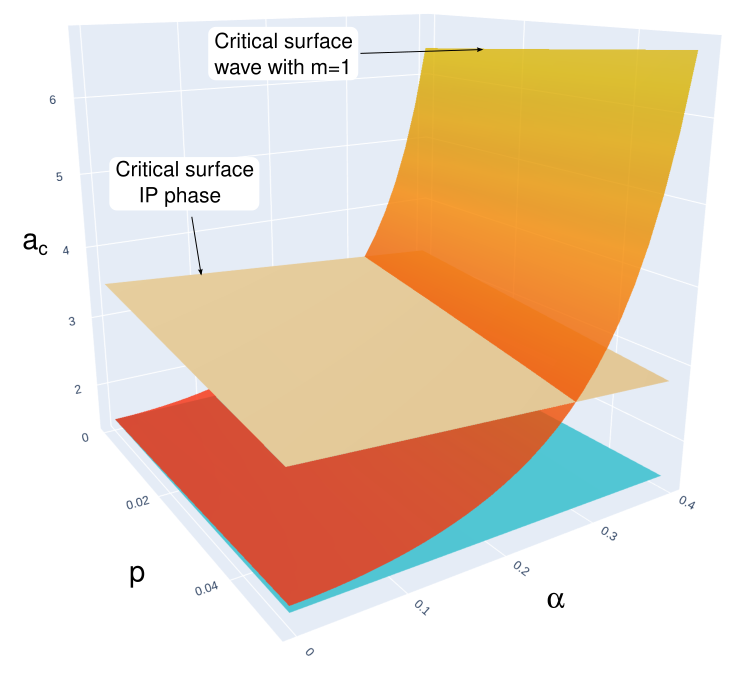
\includegraphics[width=0.45\textwidth]{fig/chap4/critical_plane_IP.png}
	\caption{
		Phase space with coordinates $(a,p,\alpha)$ and surface defined by equation~(\ref{eq:critical_plane}). In both graphs the blue
		plane has height of $a=1.5$, representing the onset of globally synchronized solutions as coupling increases. On the left, points
		above the curved surface are expected to produce stable waves with wave number $m=1$. Below this curve but above the plane, only
		globally synchronized oscillatory solutions are stable. On the right we have the same surfaces but with an additional plane
		representing a ``sketch'' of the critical surface with height $a\approx 3.1$ for the IP phase based on simulation results.
	}
	\label{fig:critical_plane}
\end{figure}

\begin{figure}
  \centering
  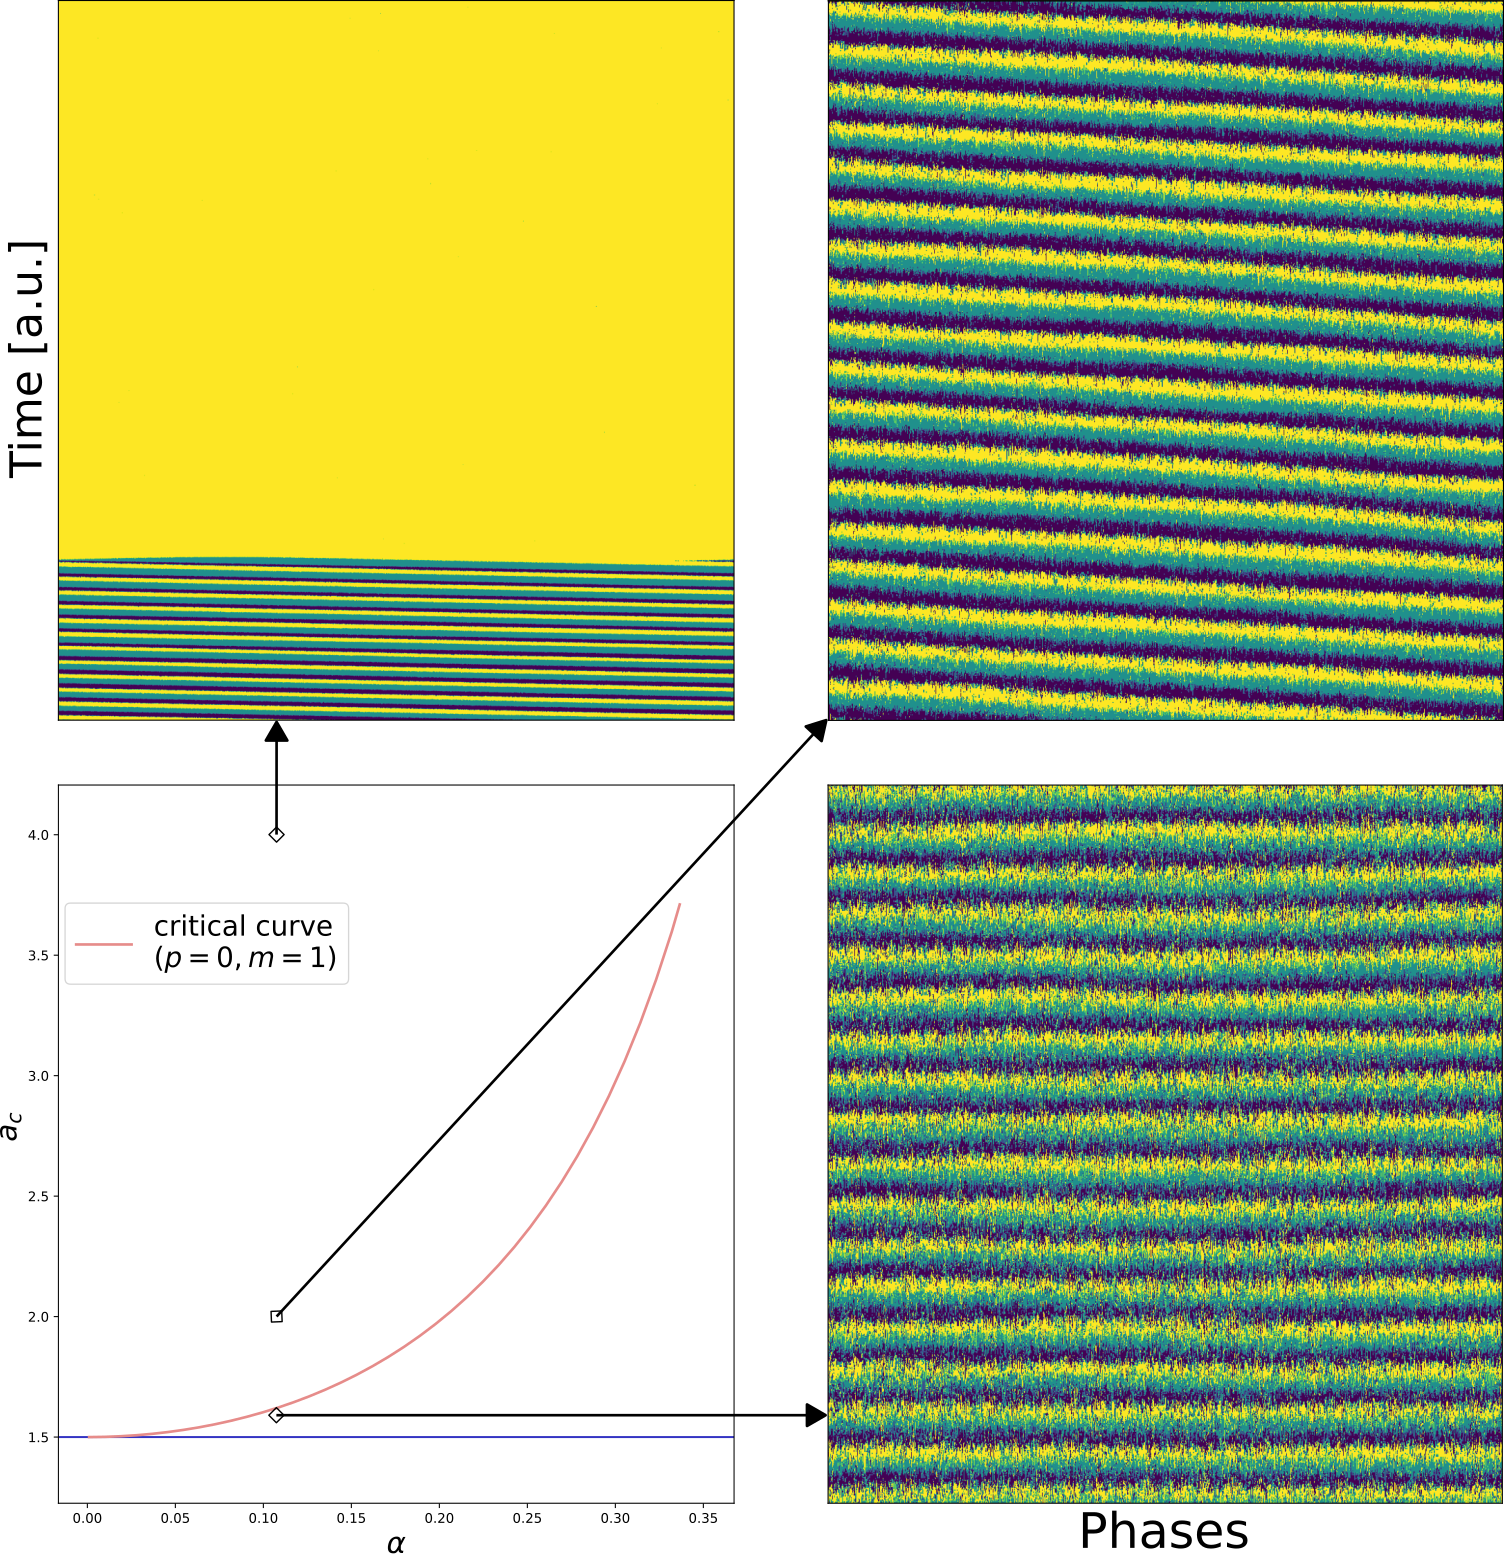
\includegraphics[width=0.8\textwidth]{fig/chap4/crit_plane_sample.png}
	\caption{
		Dynamics results from three different points in the phase space for $p=0$. Below the critical curve but above the $a=1.5$ line we
		observe global synchronized oscillations. Above the critical value for the wavenumber $m=1$ we observe the stability of the
		corresponding travelling wave while for large coupling we see the onset of the infinite period transition where the period of
		global oscillations diverges.
  }
	\label{fig:critical_plane_sample}
\end{figure}

\begin{figure}
  \centering
  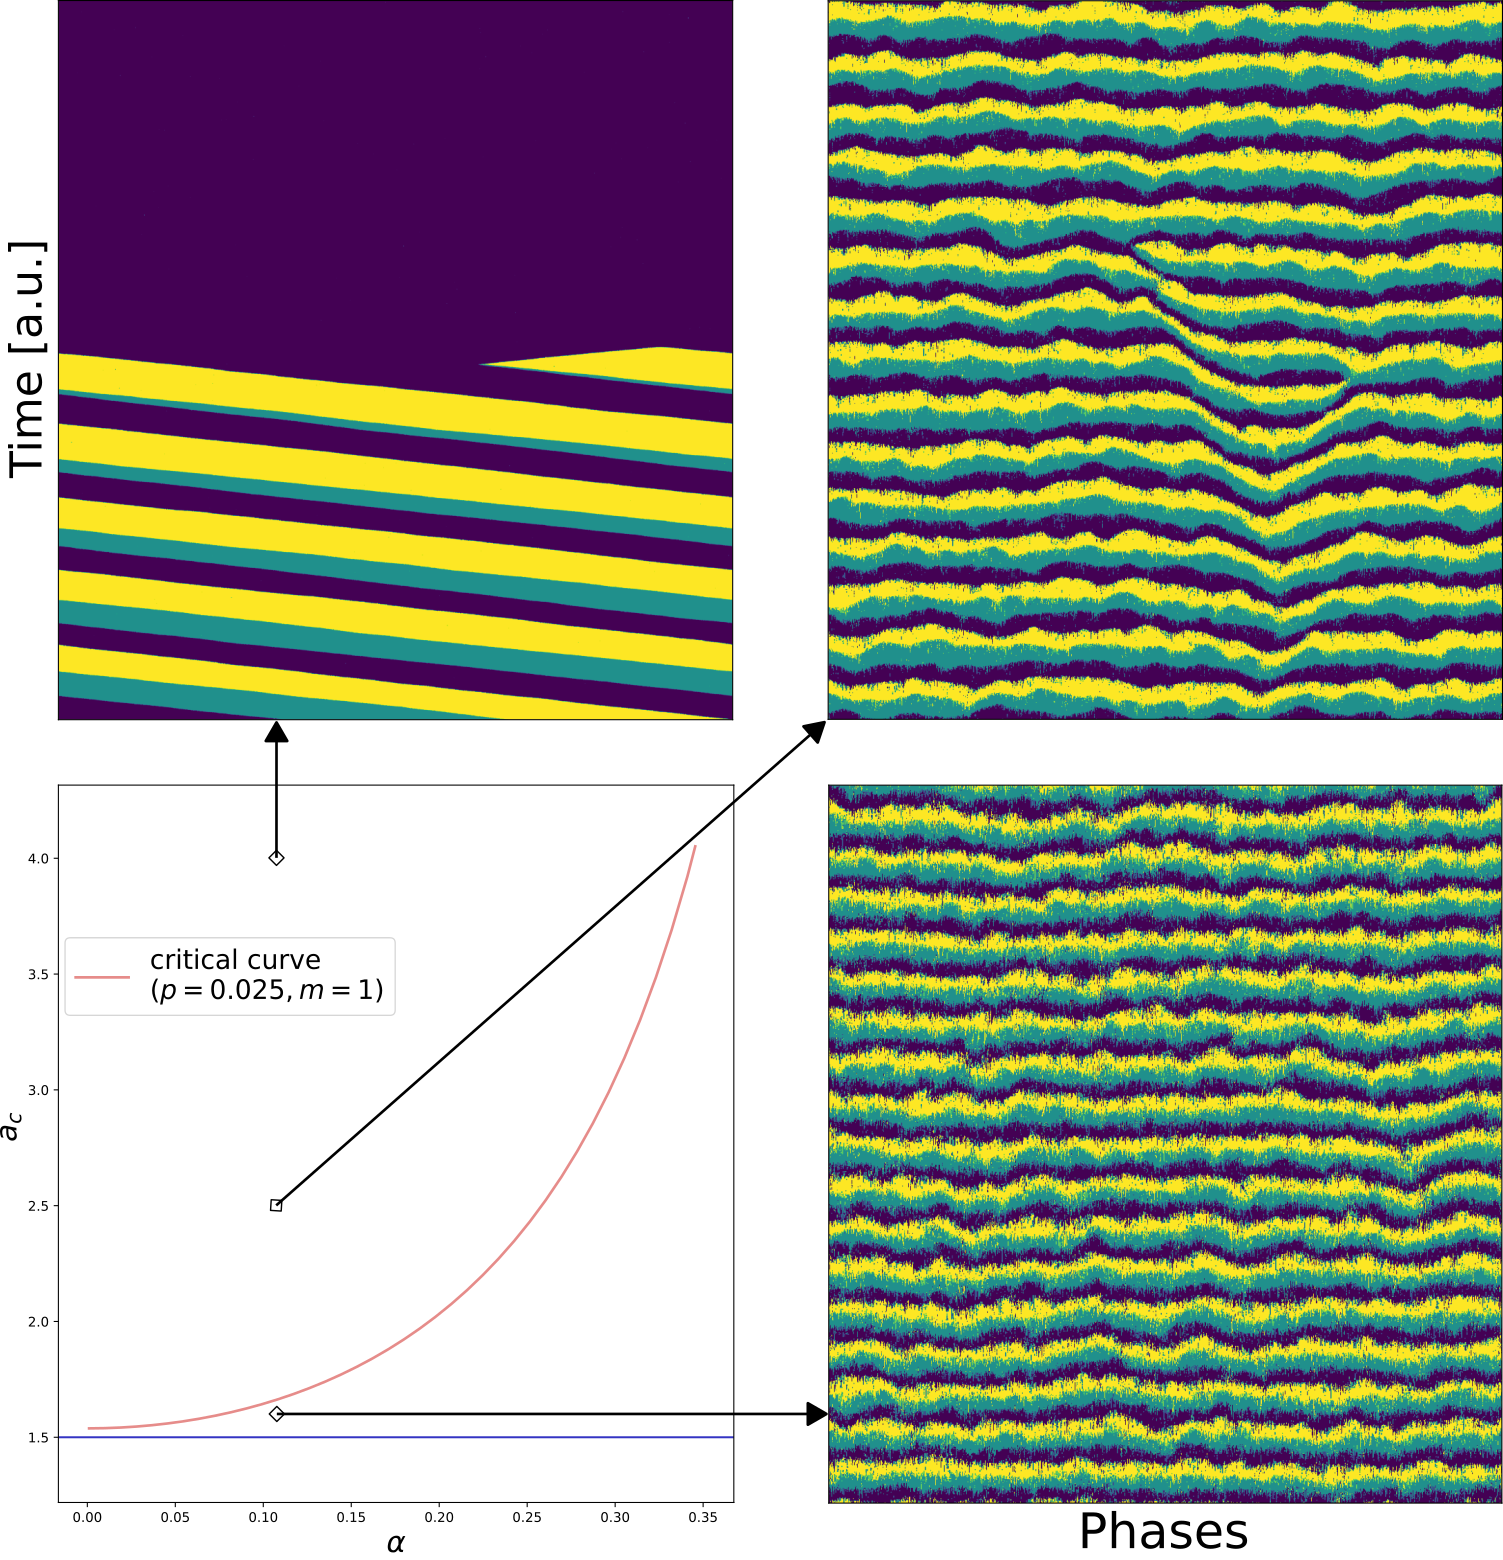
\includegraphics[width=0.8\textwidth]{fig/chap4/crit_plane_sample2.png}
	\caption{
		Dynamics results from three different points in the phase space for $p=0.025$. Below the critical curve but above the $a=1.5$ line
		we observe some global synchrony. Above the critical value for the wavenumber $m=1$ we observe intermittent stability of the
		corresponding wave, where the wave front is spontaneously created/annihilated while for large coupling we again see the onset of
		the infinite period transition.
	}
	\label{fig:critical_plane_sample2}
\end{figure}

The stability of the lowest spatial frequency wave can be tested by setting $m=1$ and performing simulations with parameters above and
below the plane defined by equation~(\ref{eq:critical_plane}) in the phase space defined by the coordinates $(a,p,\alpha)$, as seen in
figure~\ref{fig:critical_plane}. In chapter~\ref{chap:article} figure~\ref{fig:phase_diagram} we see that wave solutions are superseded
by global oscillations (GO) or the infinite period (IP) phases for sufficiently large $\alpha$, and therefore not all points above the
critical plane for wave solutions in the phase space necessarily produce stable waves. The lack of expressions for the critical
surfaces of the IP phase allows us to only sketch such surface based on the results of simulations, which show the onset of the IP
phase to remain around its complete graph ($\alpha=0.5$) value of $a\approx3.1$ (see figure~\ref{fig:chicurvespvalue}). In
figures~\ref{fig:critical_plane_sample} and \ref{fig:critical_plane_sample2} we see some examples of the unfolding of the dynamics for
six different points in the phase space. When $p=0$ the phase separations are very clean and are in accordance with predictions. In the
second case when $p=0.025$, a modestly large value, the separation becomes less abrupt, and there is a region where wave front may be
created or annihilated spontaneously. To avoid such noisy phases one would need to simulate a larger system, as the previous scaling
analysis (\ref{regularrings}) suggests, but any finite system will be subject to these fluctuations, since wave solutions will always
compete with solutions with different wave numbers. In this scenario, the globally synchronized state can be thought of as a wave
solution with wave number $m=0$, which effectively removes the spatial component of the travelling wave, leaving only oscillations in
time.

\subsection*{Spontaneous creation and annihilation of wave numbers}

\begin{figure}
  \centering
  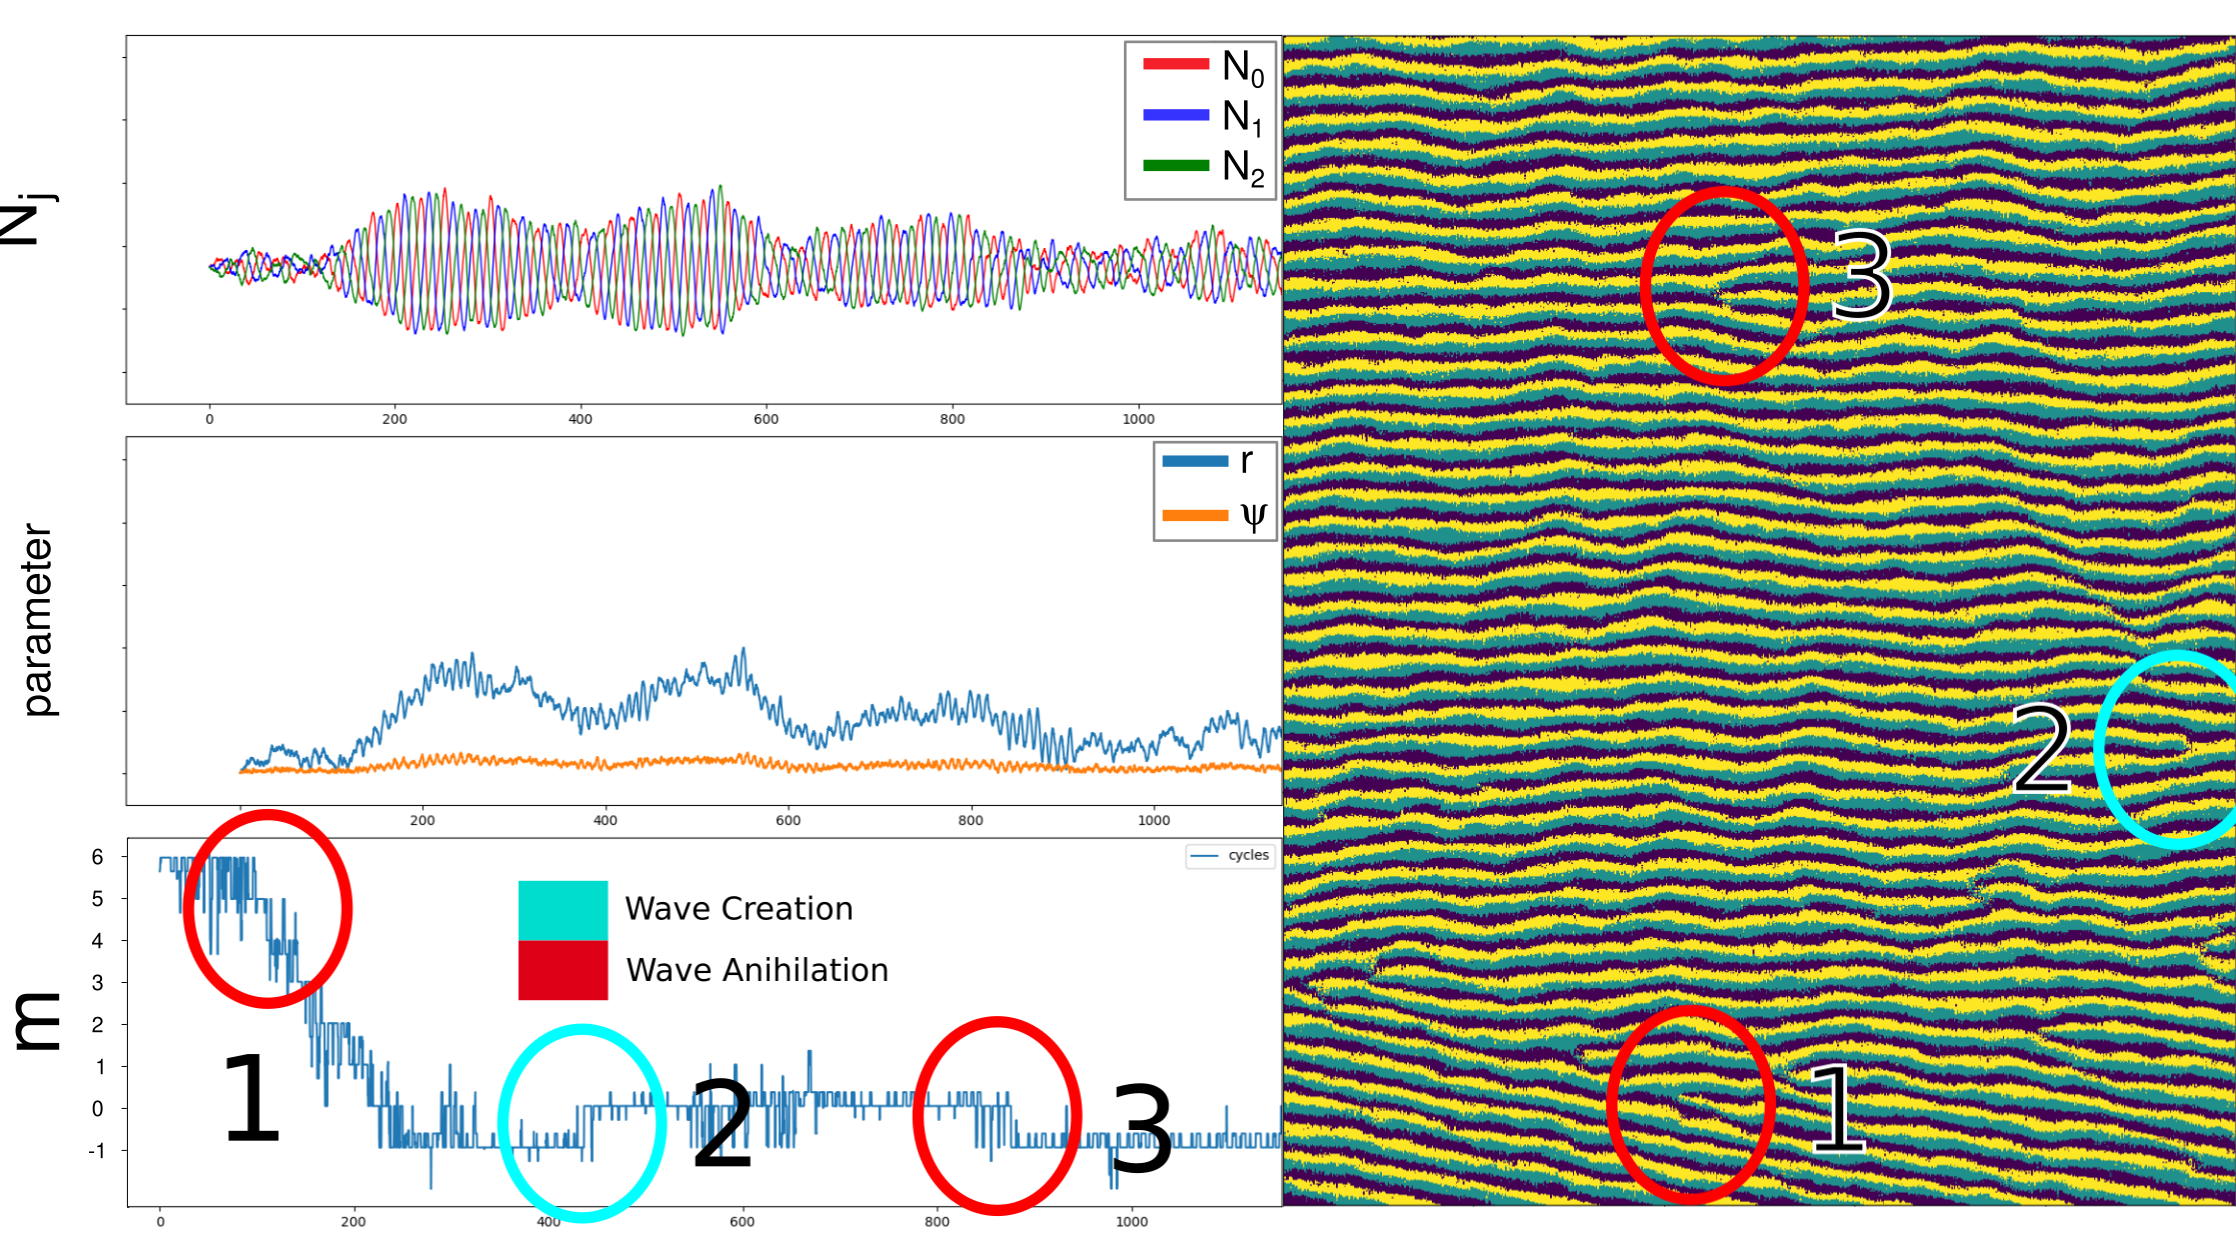
\includegraphics[width=\textwidth]{fig/chap4/annihilation.png}
  \caption{}
  \label{fig:annihilation}
\end{figure}

To illustrate how a system may fail to ever reach a steady state due to noise, we look at a simulation with parameters $(p=0.005,
\alpha=0.12, a=2.7)$ where the initial condition is a wave with wave number $m=6$. Equation~(\ref{eq:critical_plane}) tells us that the
only stable wave numbers at this point are $m=1$ and $m=2$, in addition to global oscillations $m=0$. Figure \ref{fig:annihilation}
shows that indeed the wave number quickly drops, but after reaching $m=0$ it starts oscillating around it. The value of $m=-1$ just
means the wave is actually travelling to the opposite direction compared to $m=1$, which is expected due to symmetry.

\begin{figure}
  \centering
  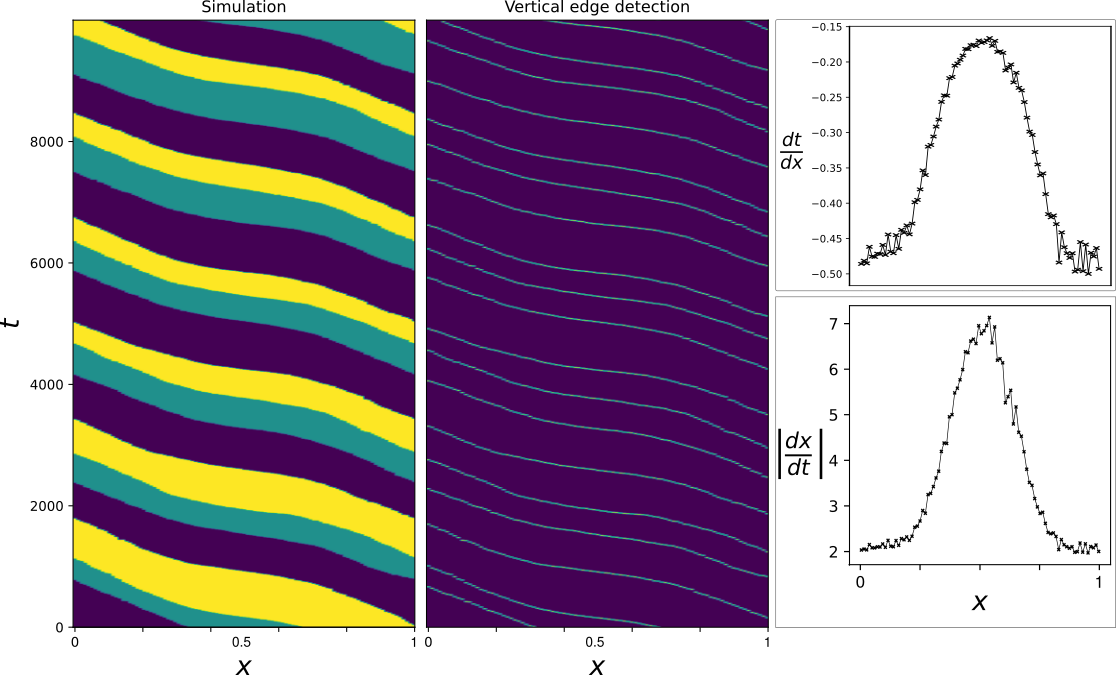
\includegraphics[width=\textwidth]{fig/chap4/speed_modulation.png}
  \caption{
		System size $N=16000$ with $\alpha=0.038$ and $p=0.0128$. Wave speed modulation generated by giving oscillators near $x=0.5$ larger
		natural frequencies, following a curve of the form $\omega(x) = 1 + 2\sin^8 \pi x$ as opposed to $\omega(x)$ being a sample of some
		unimodal distribution $g$.
  }
  \label{fig:speedmodulation}
\end{figure}

\section{Wave speed modulation}

Finally, we show that the speed of the travelling wave may be modulated by introducing biases to the oscillators natural frequencies.
In all previous simulations each oscillators natural frequency was a sample from a unimodal distribution with mean frequency around
$\bar{\omega}$. In this section we introduce a spatial bias to the natural frequencies, such that faster oscillators are near $x=0.5$
and the slower ones are located towards $x=0$ and $x=1$. In the regime of stable wave with $m=1$, the time evolution for the phase
configuration follows figure~\ref{fig:speedmodulation} for $a=3.2$, $N=8000$, $\alpha=0.038$ and $p=0.0128$. The inset on the top right
shows the value of the derivative of the wavefronts $dt/dx$. Since the wave can travel to the left or right, we take the invert this
relation and take the absolute value to get the magnitude of the wave speed, displaying a clear peak at the central region.

\section{Summary and conclusions}

Starting from Wood Cyclic Models, we have extended the investigations towards circular networks with non-global coupling by performing
extensive simulations. The general algorithm implemented in this step allowed for the investigation of arbitrary graphs, and thus it
was used to investigate small-world graphs, which were generated from these same circular graphs. At the same time, a mean-field
approximation for small-world networks was introduced, where it predicted the stability of travelling waves at positive coupling
regimes, where usually the globally synchronized solution would be observed. The limit of rewiring probability $p=0$ recovers the mean
field approximation proposed in previous works, but travelling waves were predicted to be stable even when the underlying graph has
some disorder. These wave solutions compete with global oscillations as well as with each other when there is more than one stable wave
number, leading to spontaneous creation and annihilation of wave numbers $m$. Finite systems will always be subject to these
fluctuations in wave number, but larger systems are more robust since noise becomes smaller relative to system size at the wave
boundaries. In figure~\ref{fig:speedmodulation} we see stable waves for $N=16000$ even though $p=0.0128$ consists of a relatively large
amount of disorder.

Initial simulations and scaling analysis indicated that wave solutions did not lose stability if interaction range and system size
increased proportionally to each other, a property which was captured by the MF approximation. To further strengthen the validity of
such an approximation, we tested other predictions, such as the stability of wave solutions even with the introduction of disorder
through the rewiring probability $p$ and also that the speed of propagation should increase with increasing natural frequencies.

With ongoing studies in mind, there are threads that could still be unwound. An interesting simulation that hasn't been performed yet
is how would travelling waves behave when reaching a discontinuous step in the natural frequencies, perhaps creating a reflected wave
or a series of defects as each region oscillates with a different synchronized frequency.

In more theoretical and perhaps more profound ramification is the possible connection between non-equilibrium coupled oscillators and
topological phase transitions of the Kosterlitz-Thouless type, which were hinted at on initial works by Wood et al. \cite{Wood06a} and
other independent researchers with whom I've had the opportunity to discuss this work. This speculation is based on the spatial
clustering exhibited by such systems, not only on circular graphs, where we have seen such spatial clustering and also defect
structures, but also on the 2d square lattice during the early days of the cyclic models introduction.
